%datadasedesign.tex
The database is designed in MySQL 5.1.61, and resembles the local database created by the ``Admin-group'' very closely -- the only difference is, that the Savanah database has two extra fields in the ``AuthUsers'' table: username and password. The reason for this is, that while all apps running on the android platform uses QR-codes for user authentication, this is not a fitting choice for the webinterface; it would be more complicated to scan the QR-code form a webcam to login, than to simply use a username and password combination.

\subsubsection*{Requirements}
The requirements for the database has been provided by the app groups, and are as follows:

\begin{itemize}
	\item All users must be able to login with a QR-code
	\item Each department must also be able to login
	\item All users must be linked to at least one department
	\item All guardians must be able to be linked to at least one child.
	\item All parents must be able to be linked to at least one child.
	\item All users must be able to have access all the apps
	\item All users must be able to access their own pictures, and all public pictures
	\item All departments must be able to access all public pictures
	\item All pictures needs to be able to be linked to different tags
	\item Pictures must be able to be linked with audio and vice versa
	\item A department must be able to have a subdepartment\footnote{Example: ``Birken'' has two departments, at two different addresses, both these subdepartments needs to be linked with ``Birken'' as a superdepartment}
\end{itemize}

\subsubsection*{Diagram}
A database diagram has been made to get a overview of the different tables and their relations. This diagram is designed in DIA, which is a GTK+ based diagram creation program\cite{Dia}, and can be seen in \autoref{fig:DiaDesign}.

\begin{figure}[htbp]
	\centering
		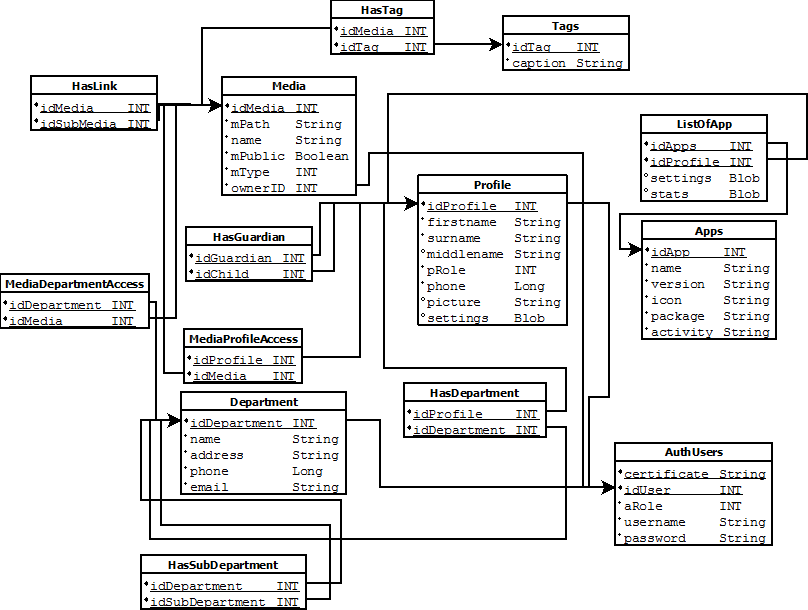
\includegraphics[width=1.00\textwidth]{images/DiaDesign.png}
	\caption{Dia diagram of the database}
	\label{fig:DiaDesign}
\end{figure}

Although the diagram in \autoref{fig:DiaDesign} does not meet the standard of database diagrams, it does provide a good view of the different tables, and the relations: Foreign keys points to where the value is fetched form. This crude diagram shows that be having the ``idUser'' from the ``AuthUsers'' one is able to access all other information for that specific user.

\subsubsection*{Rules}
To provide the security needed in the system, a few rules need to apply for the databse:
\begin{itemize}
	\item The ``Profile''$\rightarrow$''AuthUsers'' relation must be one-to-one, as one user form the ``AuthUsers'' can only have one profile in the system
	\item The ``Department''$\rightarrow$''AuthUsers'' relation must be one-to-one, as one department form the ``AuthUsers'' can only be one department in the system
	\item The ``idUser'' in ``AuthUsers'' must be unique.
	\item The ``username'' in ``AuthUsers'' must be unique
	\item It must be possible to distinguish between users and departments in the ``AuthUsers'' table
	\item It must be possible to distinguish between children, parents and guardians in the ``Profile'' table
\end{itemize}

These rules will be applied in a mix between SQL script and software level in \textbf{REF TIL SECTION}